\chapter{Introduction}
\label{cpt:intro}

Static cameras that observe the same scene for a long period of time can give us valuable information, such as clues for geo-location\cite{jacobs08geoorient}.  Given such a sensor, how can we help users to understand the variation in the scene?  This project explores automatic visualization tools to quickly show interesting variation.  As opposed to natural variation, such as day vs. night or sunny days vs. cloudy days, unnatural variation is less predictable and more interesting.  People, cars, and other objects in the scene give more high level semantic information, and to understand a scene is to understand this variation.


\section{AMOS Dataset}

\begin{figure}[ht]
\centering
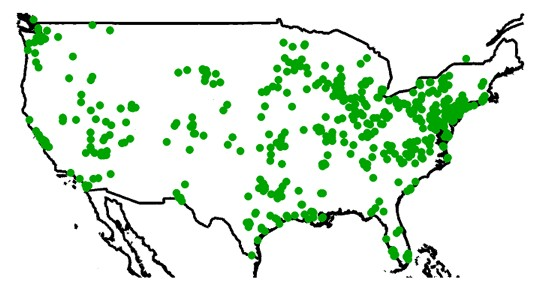
\includegraphics[width = 1\textwidth]{figures/localizationMap.jpg}
\caption[Map of known webcam locations from the AMOS dataset.]{Many of the AMOS webcams are located in the United States, as shown in this map.}
\label{fig:localizationMap}
\end{figure}

The Archive of Many Outdoor Scenes (AMOS) consists of over 3,000 webcams, 1,020 of which we have been actively capturing every half hour for the last three years.  In this time, we have amassed 35,376,886 images, totaling roughly 868 gigabytes of data.  Most of the cameras are from the USA, many of which are plotted in Figure \ref{fig:localizationMap}.  Clearly, it is impractical to maintain and understand such a large dataset without help.  We need to automatically present users with visualizations of this variation.



\section{Outline of the Paper}

We have many images from which we need to find interesting variants.  A lot of the variance is natural and controlled - day to night transitions, seasonal changes, and weather are all predictable and easy to lean.  First, we will present the mathematical tool Principal Component Analysis (PCA) as an algorithm to learn this natural variation.  Next, we will discuss different inputs to the PCA algorithm to best capture our goal.  Finally, we will show several visualization tools and evaluation criteria, and discuss their success in capturing PCA error, which is the interesting variation for which we search.


